\section{Experiments}
\subsection{Dataset and chronological split}
UCI Online Retail records transactions at a UK-based non-store retailer between 1 December 2010 and 9 December 2011. The business sells gifts and includes wholesale customers~\citep{chen2015}; invoice-level associations should not automatically be interpreted as individual household preferences. The relevant fields are invoice number, product code, timestamp, quantity, unit price, customer identifier and country. Dates are used as recorded; no undocumented timezone conversion is applied.

\begin{figure}[!htbp]
\centering
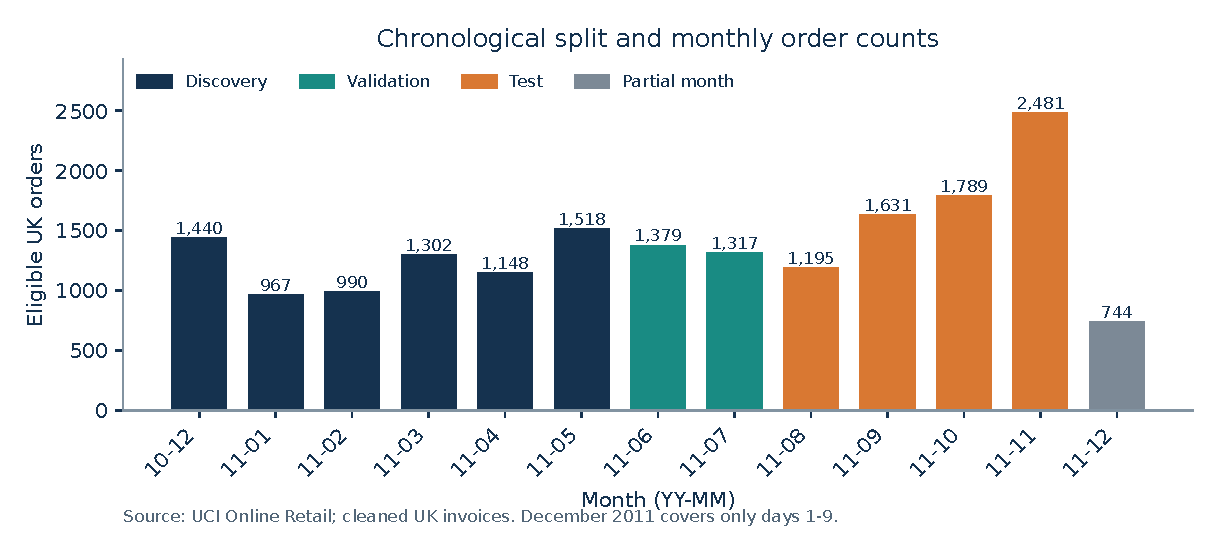
\includegraphics[width=\linewidth]{01_monthly_orders.pdf}
\caption{Eligible UK orders and the chronological evaluation design. The final December is incomplete and excluded from the main comparison.}
\label{fig:orders}
\end{figure}

\begin{table}[!htbp]
\centering
\begin{tabular}{llr}
\toprule
Partition & Inclusive calendar months & UK orders\\
\midrule
Discovery & December 2010--May 2011 & \TrainOrders\\
Validation & June--July 2011 & \ValidationOrders\\
Held-out test & August--November 2011 & \TestOrders\\
\bottomrule
\end{tabular}
\caption{Orders are neither shuffled nor split across time partitions.}
\end{table}

\subsection{Settings and selection protocol}
\label{sec:settings}
The discovery grid combines minimum supports of 0.5\%, 1\% and 2\% with minimum confidences of 30\%, 50\% and 70\%. Discovery lift must be at least 1.2. The selected setting maximizes mean June--July retention under the common monthly requirements, subject to at least 20 discovery rules. Ties prefer more rules, then higher support, then higher confidence. The 20-rule floor is a project coverage choice, not a statistical significance criterion; its effect is examined explicitly.

The winning setting is 2\% discovery support and 50\% confidence, producing \SelectedRules{} rules with \ValidationRetention{} validation retention. No test month is used to select this setting. All nine predeclared configurations are later evaluated for descriptive sensitivity analysis; these test results do not trigger reselection. The partial December 2011 metrics are saved separately and are not used in the principal claims.

The discovery window is deliberately longer than each evaluation window. It supplies observations for candidate mining, while the month is the unit of persistence assessment. The lower monthly support gate is shared by every discovery configuration; it is not retuned to an individual month or rule.


\subsection{Algorithm equivalence and computational cost}
The benchmark uses \TrainOrders{} discovery orders encoded over 1,409 products. The shared Boolean matrix occupies about 9.9 MiB. Each algorithm-support pair runs in three fresh Python processes, alternating method order between repetitions. The timer covers frequent-itemset mining only, excluding process startup, data loading, encoding, rule generation and result serialization. Memory is the peak working set of the worker process, including its interpreter and input matrix, rather than an algorithm-only allocation estimate.

\begin{figure}[!htbp]
\centering
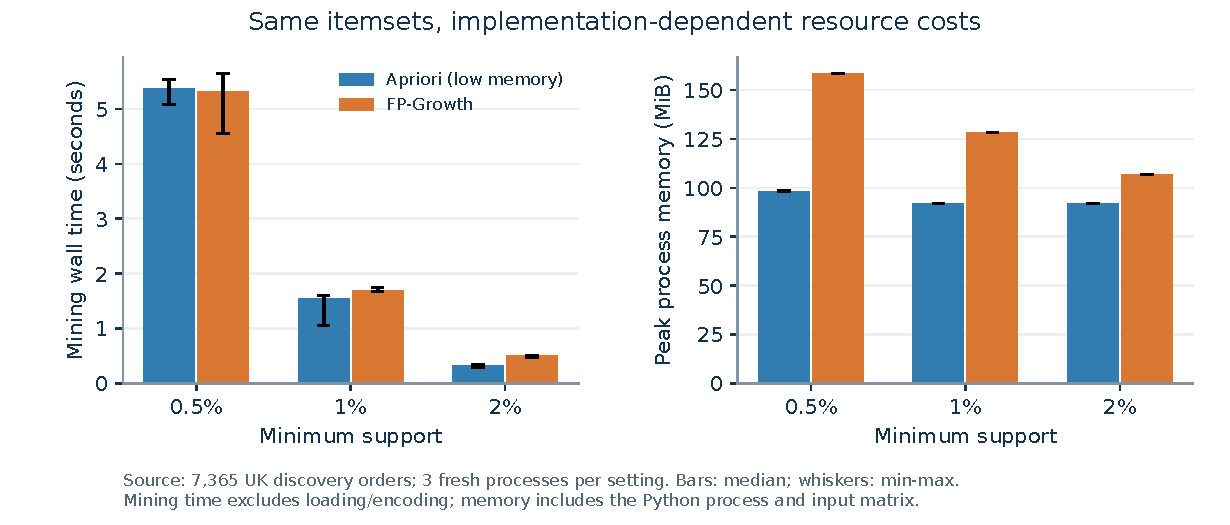
\includegraphics[width=\linewidth]{02_benchmark.pdf}
\caption{Measured resource use on the local AMD Ryzen 9 7940H computer with approximately 64 GB RAM. These are implementation-level comparisons, with Apriori low-memory mode enabled.}
\label{fig:benchmark}
\end{figure}

\begin{table}[!htbp]
\centering\small
\begin{tabular}{llrrrr}
\toprule
Support & Method & Median s & Range s & Peak MiB & Itemsets \\
\midrule
0.5\% & Apriori LM & 5.372 & 5.078--5.541 & 98.2 & 20,906 \\
0.5\% & FP-Growth & 5.320 & 4.560--5.654 & 158.5 & 20,906 \\
1.0\% & Apriori LM & 1.541 & 1.048--1.610 & 92.1 & 2,218 \\
1.0\% & FP-Growth & 1.695 & 1.671--1.744 & 128.4 & 2,218 \\
2.0\% & Apriori LM & 0.323 & 0.294--0.341 & 92.2 & 413 \\
2.0\% & FP-Growth & 0.501 & 0.470--0.502 & 106.7 & 413 \\
\bottomrule
\end{tabular}

\caption{Three-process timing ranges and median peak process memory. ``LM'' denotes low-memory mode. All repeated outputs have identical canonical signatures at a given support.}
\end{table}

Both algorithms return exactly the same bounded frequent itemsets and support counts: 20,906 itemsets at 0.5\% support, 2,218 at 1\%, and 413 at 2\%. At 0.5\%, their median times are close and their observed ranges overlap. Apriori is faster in these runs at the higher thresholds. This does not contradict FP-Growth's algorithmic motivation: library implementation, short maximum pattern length, input representation and dataset structure all affect measured performance. Three repetitions on a shared laptop do not establish a universal speed ranking.

The largest benchmark worker peak is \MaxBenchmarkMemory{} MiB. The core experiment, including parameter evaluation and rolling windows, takes approximately \ExperimentSeconds{} seconds on this run; workbook preparation and document rendering are outside that timing. These observations support local feasibility for the declared settings, not an unrestricted low-support search.

The comparison is paired by input and support, while separate processes still share the laptop's operating-system load. Alternating method order reduces dependence on a fixed execution sequence, and the ranges expose observed timing variability. The measured memory differences describe these library implementations and settings; they do not estimate asymptotic space complexity.


\subsection{Temporal retention of the frozen cohort}
\begin{figure}[!htbp]
\centering
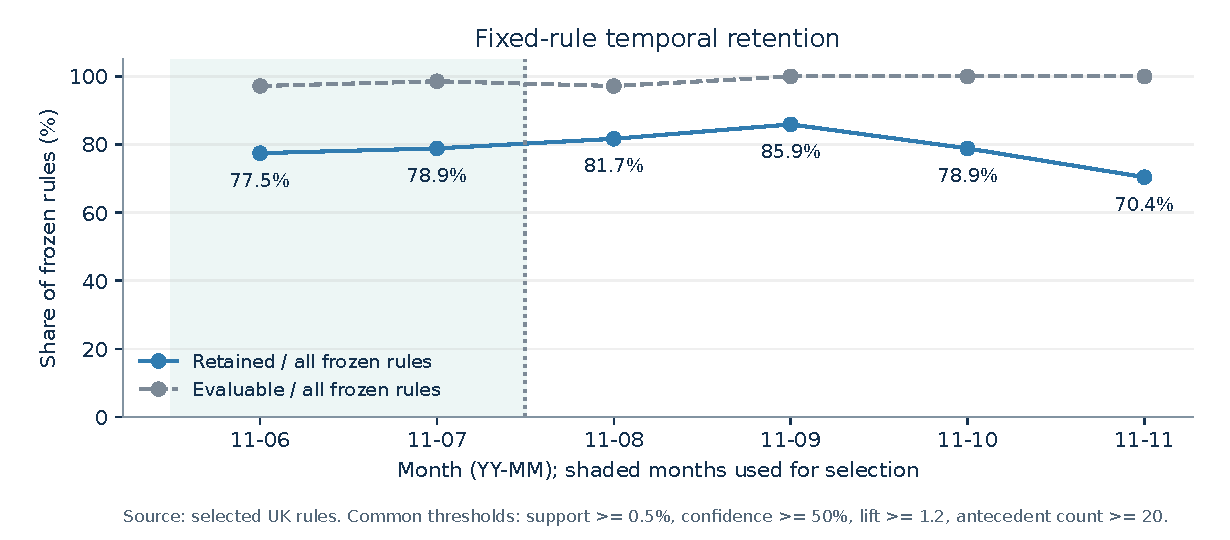
\includegraphics[width=.95\linewidth]{03_temporal_retention.pdf}
\caption{A fixed cohort of \SelectedRules{} rules is followed through validation and held-out months. Coverage is plotted separately to distinguish insufficient evidence from failure of the metric thresholds.}
\label{fig:retention}
\end{figure}

\begin{table}[!htbp]
\centering\small
\begin{tabular}{lrrrr}
\toprule
Month & Orders & Evaluable & Retained & Retention \\
\midrule
2011-08 & 1,195 & 69/71 & 58/71 & 81.7\% \\
2011-09 & 1,631 & 71/71 & 61/71 & 85.9\% \\
2011-10 & 1,789 & 71/71 & 56/71 & 78.9\% \\
2011-11 & 2,481 & 71/71 & 50/71 & 70.4\% \\
\bottomrule
\end{tabular}

\caption{Held-out results with all \SelectedRules{} discovered rules retained in each denominator.}
\end{table}

Mean test retention is \MeanRetention{} (\RetainedRuleMonths/\RuleMonths{} rule-months), while evaluability is \Coverage{}. The gap is therefore primarily failure of the metric requirements for observed rules, rather than missing products or small antecedent counts. Of 59 unsuccessful rule-months, a sequential failure attribution assigns 54 to confidence below 50\%, three to support below 0.5\%, and two to insufficient antecedent count. These categories describe which criterion fails first, not causes of purchasing behavior.

\begin{figure}[!htbp]
\centering
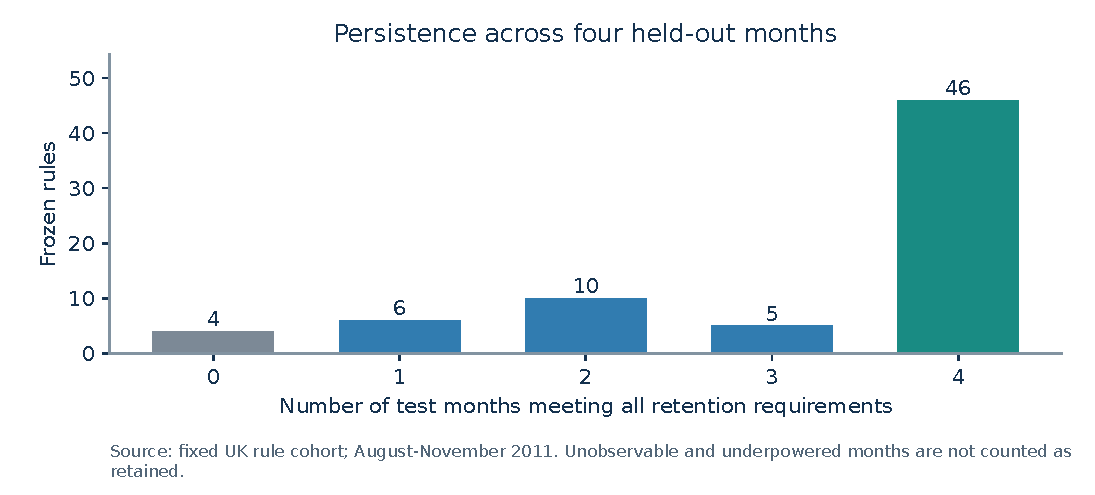
\includegraphics[width=.75\linewidth]{05_persistence.pdf}
\caption{Persistence distribution within the frozen cohort. The 46 rules retained in all four test months are a stronger descriptive notion of stability than a single-month success.}
\label{fig:persistence}
\end{figure}

Retention is not monotonic: it rises from 81.7\% in August to 85.9\% in September, then falls to 78.9\% in October and 70.4\% in November. Four rules never satisfy all requirements in the test period.

September and November both have complete rule evaluability, yet retention falls from 61 to 50 rules while order volume rises from 1,631 to 2,481. The decline therefore cannot be explained by the antecedent-count gate alone.


\subsection{Threshold sensitivity and observability}
\begin{figure}[!htbp]
\centering
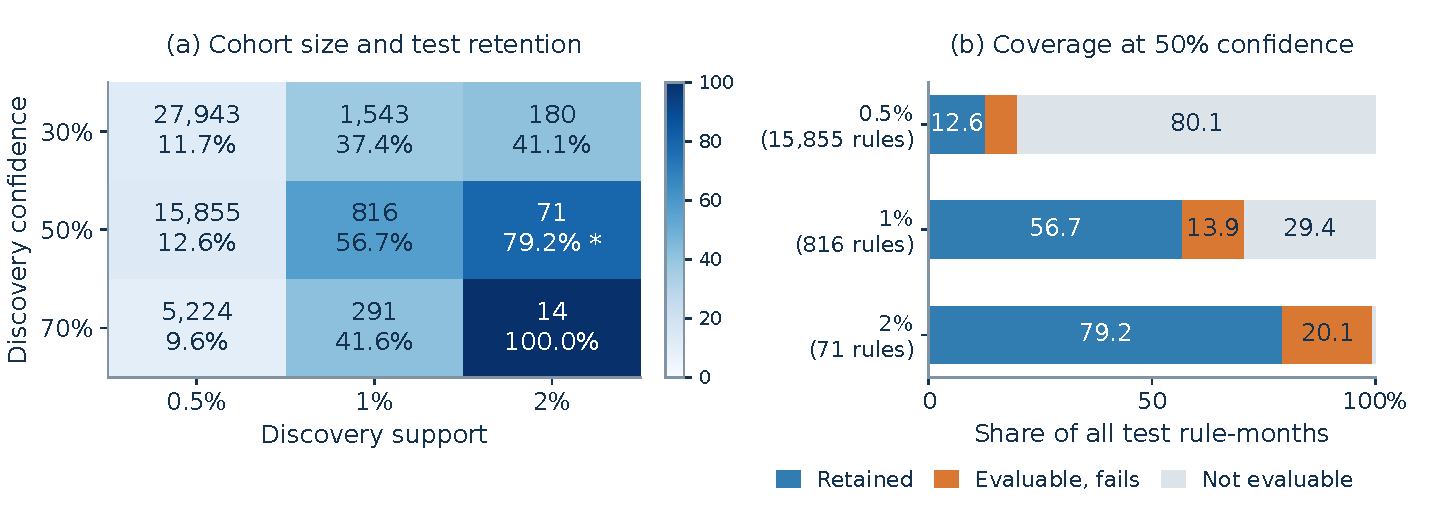
\includegraphics[width=\linewidth]{09_threshold_observability.pdf}
\caption{\textbf{Rule quantity and evidence availability.} (a) Cell entries give rule count and mean test retention; the asterisk marks validation-only selection. (b) With discovery confidence fixed at 50\%, all test rule-months are partitioned into retained, evaluable but failing a metric gate, and not evaluable. All cohorts use the same monthly criteria; test-grid comparisons are descriptive.}
\label{fig:thresholds}
\end{figure}

Increasing the discovery support threshold reduces the rule set and generally improves its evaluability. For example, with 50\% discovery confidence, the 0.5\% support setting produces 15,855 rules but only 19.9\% of their test rule-months are evaluable. Overall retention is 12.6\%, compared with 63.2\% conditional retention among evaluable observations. The primary 2\% support setting has 99.3\% coverage and 79.2\% overall retention. The difference must not be attributed entirely to changing customer behavior: lower-support discovery patterns frequently lack the minimum monthly evidence.

Raising confidence alone does not guarantee better operational retention. At 1\% discovery support, the 70\% confidence cohort has 41.6\% overall retention and 42.2\% coverage; its conditional retention is 98.6\%. The high confidence screen can therefore identify precise but rarely observable associations. Adequate support is central when moving from a six-month discovery window to individual months.

\begin{table}[!htbp]
\centering\small
\begin{tabular}{lrrr}
\toprule
Rule floor & Selected rules & Validation retention & Test retention \\
\midrule
10 & 14 & 100.0\% & 100.0\% \\
20 & 71 & 78.2\% & 79.2\% \\
50 & 71 & 78.2\% & 79.2\% \\
100 & 816 & 55.5\% & 56.7\% \\
\bottomrule
\end{tabular}

\caption{Post-hoc sensitivity of the minimum-rule constraint. Each row still selects by validation scores only; the primary result remains the predeclared 20-rule policy.}
\label{tab:floor}
\end{table}

The 14-rule setting at 2\% support and 70\% confidence attains 100\% observed validation and test retention, but does not satisfy the primary 20-rule floor. With a floor of 100, selection instead yields 816 rules and 56.7\% test retention. Consequently, the 71-rule result is conditional on the chosen coverage objective; it is not presented as a uniquely optimal retail policy or a guarantee of future persistence.


\subsection{Representative persistent and fragile associations}
\begin{figure}[!htbp]
\centering
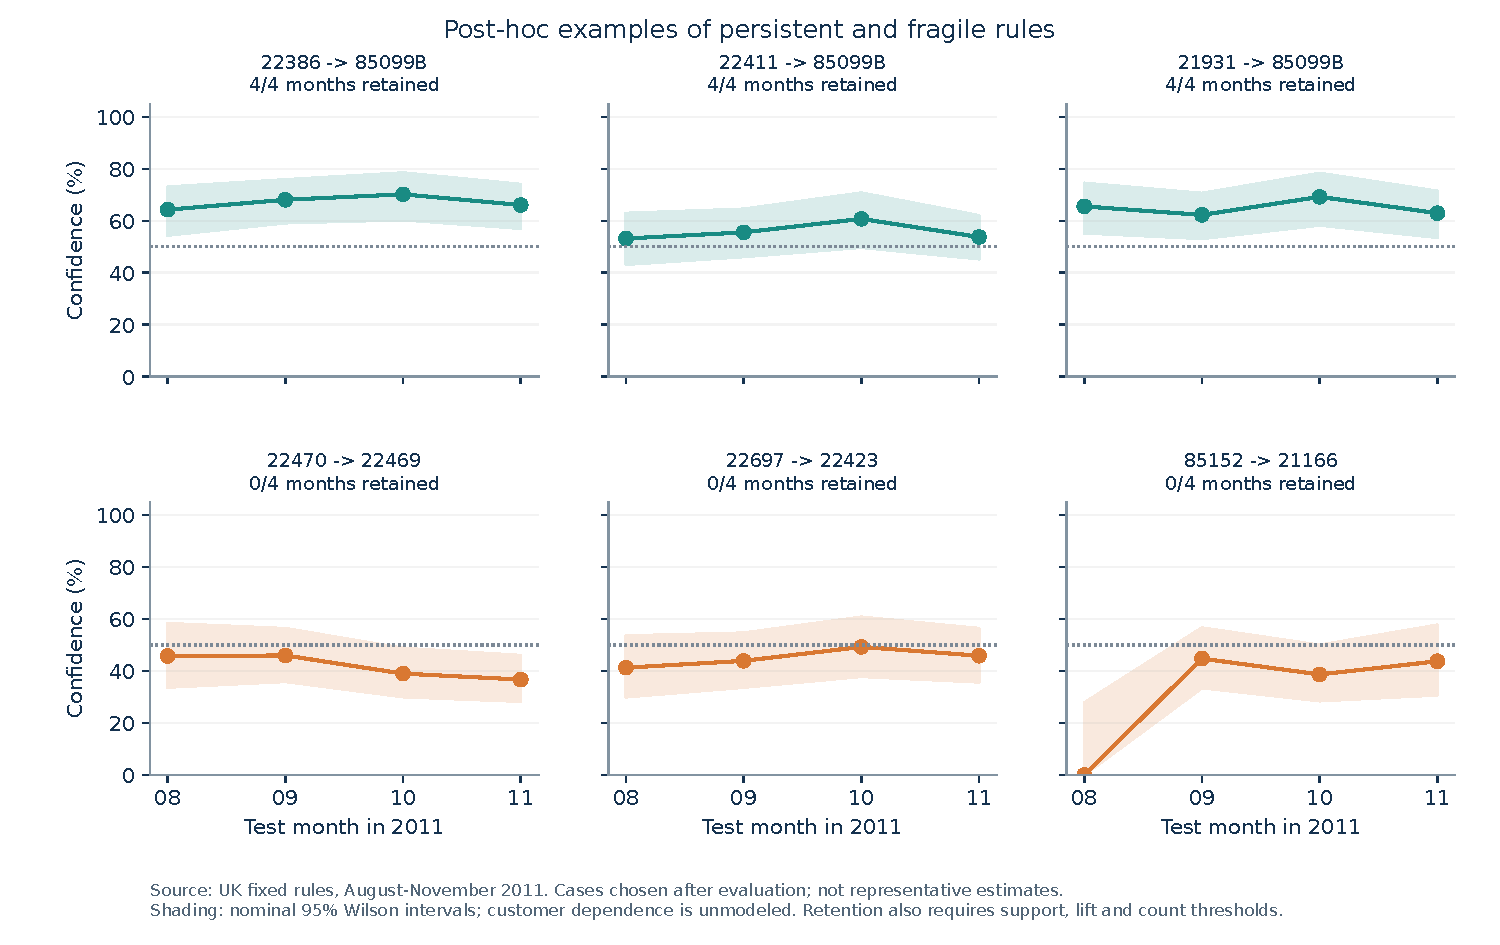
\includegraphics[width=\linewidth]{06_case_studies.pdf}
\caption{Illustrative cases selected after evaluation: the three most persistent rules are ranked by minimum monthly antecedent count, and the least persistent by discovery confidence. Bands are nominal 95\% Wilson intervals for confidence. They do not adjust for repeated customers, dependent rules or multiple comparisons.}
\label{fig:cases}
\end{figure}

The rule \texttt{22386}$\rightarrow$\texttt{85099B} connects the pink polkadot jumbo bag to the red retrospot jumbo bag. Discovery confidence is 67.3\%; its test-month mean is 67.2\%, and its lowest monthly confidence is 64.3\%. At least 94 antecedent-containing orders occur in each test month. Together with the support and lift requirements, this provides a clear example of persistence within the observed population.

In contrast, \texttt{22470}$\rightarrow$\texttt{22469}, linking the large wicker heart to the small wicker heart, has 62.4\% discovery confidence but only 41.9\% average test confidence. It is evaluable in all four test months yet retained in none. Its mean test lift remains approximately 7.47, illustrating that strong lift can coexist with confidence below the operational target. A second fragile case, \texttt{85152}$\rightarrow$\texttt{21166}, also has one month with insufficient antecedent evidence.

Product names are taken from the most common description in the discovery data. The examples illustrate the retained and failed categories; because they were chosen using observed outcomes, they are not an unbiased sample for estimating a general success rate. The complete per-rule table supports inspection beyond these cases. There is no promotion, inventory or pricing-policy history that could establish why a particular association changed.


\subsection{Population and rolling-window checks}
\begin{figure}[!htbp]
\centering
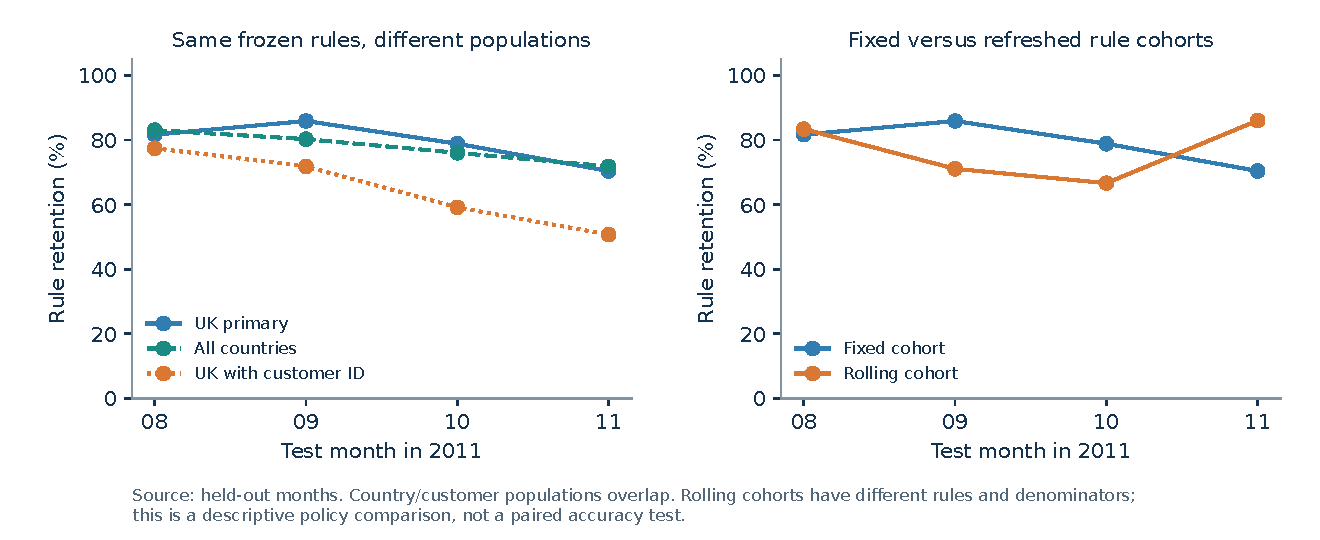
\includegraphics[width=\linewidth]{07_robustness.pdf}
\caption{Population checks retain the same frozen UK rules. Rolling three-month discovery instead produces a different cohort before each test month, using the already selected thresholds. Those cohorts have different denominators and are not a paired accuracy comparison.}
\label{fig:robustness}
\end{figure}

\begin{table}[!htbp]
\centering\small
\begin{tabular}{lr}
\toprule
Evaluation population & Mean monthly retention \\
\midrule
UK primary & 79.2\% \\
All countries & 77.8\% \\
UK with customer ID & 64.8\% \\
UK at most 100 products & 62.3\% \\
\bottomrule
\end{tabular}

\caption{Mean August--November retention of the same 71 rules. The basket-size restriction is a post-hoc diagnostic; the primary population and selection are unchanged.}
\label{tab:populations}
\end{table}

The population effect is material. Orders lacking a customer identifier are much larger on average in the test months: their monthly means range from 98.2 to 182.0 distinct products, versus 20.1 to 24.9 for orders with an identifier. Removing orders with more than 100 products reduces retention to \SmallBasketRetention{}. This is evidence that order composition matters, not proof that missing identifiers or large baskets cause instability. The subsets overlap, and the rule cohort was selected on the full UK discovery population.

Rolling discovery yields 265, 481, 489 and 201 rules for August through November, with next-month retention of 83.4\%, 71.1\%, 66.7\% and 86.1\%. Refreshing does not uniformly improve the retained fraction. It can expand the available cohort, but a comparison of business value would also need rule coverage, utility and implementation costs. The monthly cohorts and their overlaps with the fixed set are saved in the experiment outputs.

Only 46, 50, 48 and 37 of the original 71 rules reappear in the corresponding rolling cohorts. Thus refreshing changes which relationships are proposed, as well as the period from which their statistics are estimated. A larger refreshed cohort can contain many new rules while omitting some originally selected ones. Its retention rate answers a policy-level question about that new cohort, rather than whether the original associations have improved. A prospective comparison would need the same target orders and a predefined recommendation budget, together with explicit measures of product coverage and utility.
